
\chapter{Interface graphique}

La majeure partie du code que nous avons développé traite du chargement des données 
en mémoire, de leur traitement, du calcul des features et de la classification grâce 
aux algorithmes proposés par \tcode{scikit-learn} et \tcode{keras}.
Néanmoins toute cette partie du code n'est pas très visuel et nous avons 
décidé de créer une petite interface graphique pour rendre le tout plus attrayant.
Nous avons créer deux widgets avec la bibliothèque \tcode{PyQt}, un \nfw{binding}
Python du très connu framework Qt écrit en \Cpp.
\begin{itemize}
  \item un widget permettant de visualiser les données MNIST;
  \item un widget permettent la saisie d'un chiffre et sa reconnaissance.
\end{itemize}


\section{Visualisation des données}

Ce widget permet de visualiser les données MNIST, que ce soit du jeu d'entraînement 
ou du jeu de test.

\begin{figure}[h]
  \centering
  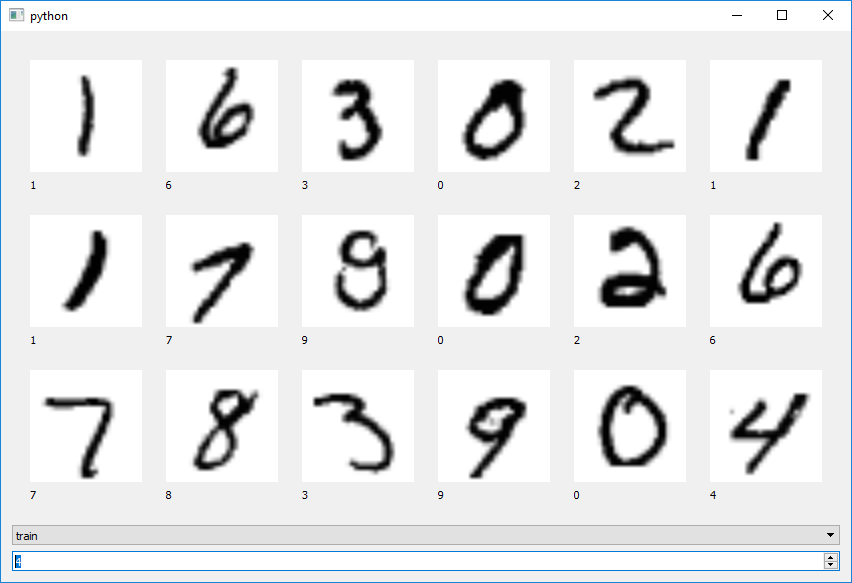
\includegraphics[scale=0.66]{assets/dataset-widget}
  \caption{Widget de visualisation des images.}
\end{figure}

Une liste déroulant permet de sélectionner le jeu de données.
L'affichage se fait sous forme de pages. 
Il est affiché en dessous de chaque image le chiffre correspondant.

Ce widget est intéressant car il permet de se rendre compte assez rapidement que 
certaines images de MNIST sont très difficiles à reconnaître. 
Un taux de reconnaissance supérieur à 95\% est donc déjà très satisfaisant.
Cela pose également la question de la pertinence de certaines images 
pour l'entraînement des réseaux de neurones : ne vaudrait-il pas mieux 
retirer certaines images qui ne ``méritent'' pas d'être reconnues ?


\section{Reconnaissance de caractères}

Ce deuxième widget permet à l'utilisateur de dessiner à la souris des chiffres 
et de les soumettre à certaines méthodes de reconnaissance présentées précédemment.

\begin{figure}[h]
  \centering
  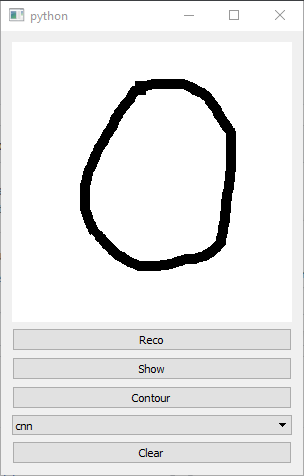
\includegraphics[scale=0.66]{assets/draw-widget}
  \caption{La note que l'on espère ne pas avoir.}
\end{figure}

L'appuie sur le bouton \textsc{reco} envoie l'image au classifieur sélectionné 
et affiche les trois chiffres les plus probables.

\begin{figure}[h]
  \centering
  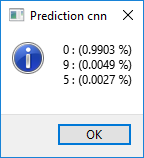
\includegraphics[scale=0.9]{assets/prediction-widget}
  \caption{Probabilités données par le réseau convolutif.}
\end{figure}

En pratique, on se rend compte que le réseau convolutif est le meilleur, et de loin.
En effet, ce dernier a été entraîné avec un jeu de données augmenté tandis que les autres 
ont seulement utilisés les images du jeu de MNIST qui sont centrées et relativement de 
même taille.
Comme l'utilisateur a tendance à faire des chiffres un peu plus gros (ou plus petit) 
que ceux de MNIST et pas forcément centrés, le taux de reconnaissance est assez faible.
D'après nos essais, le réseau convolutif a un taux de reconnaissance tout à fait 
satisfaisant.